\documentclass{article}

\usepackage[english]{babel}
\usepackage[a4paper,top=2cm,bottom=2cm,left=3cm,right=3cm]{geometry}

\usepackage{amsmath}
\usepackage{graphicx}
\usepackage{booktabs}
\usepackage{hyperref}
\usepackage{microtype}
\usepackage{subcaption}

\hypersetup{colorlinks=true, linkcolor=blue, citecolor=blue, urlcolor=blue}

\title{High-Performance Cholesky Factorization with OpenMP\\
       \large MPhil Data Intensive Science --- C2 High Performance Computing}
\author{Basia Koch \\ University of Cambridge}
\date{\today}

\begin{document}

\maketitle

\begin{abstract}
An in-place Cholesky factorization routine $C = LL^T$ is developed in C and
optimized in five stages for a single 76-core CSD3 icelake node.
Loop interchange and compiler flags (\texttt{-O3 -march=native -ffast-math})
yield a 13--16$\times$ single-thread improvement over the \texttt{-O0} baseline.
A flat OpenMP parallelization reaches at most 46.5~GFLOP/s at 48~threads for
$n=2000$, then \emph{degrades}, because $O(n)$ barriers dominate at high thread
counts.
Restructuring into a right-looking panel-blocked algorithm (panel width
$\mathrm{NB}=96$) reduces barrier count from $n$ to $\lceil n/\mathrm{NB}\rceil$,
giving 59.4$\times$ speedup and 78.2\% efficiency at 76~threads for $n=8000$
(146.9~GFLOP/s).
Four microarchitectural optimizations---column packing, private L11 cache,
4-wide SYRK unrolling, and round-robin scheduling---add a 2.53$\times$
single-thread gain, reaching 181.2~GFLOP/s at 76~threads.
\end{abstract}

% ======================================================================
\section{Introduction}
% ======================================================================

Cholesky factorization $C = LL^T$ is a core operation in Bayesian inference,
Gaussian-process regression, and numerical optimization, where it is used to
invert and compute the determinant of symmetric positive-definite covariance
matrices.
For $n$ observations, the covariance matrix $C \in \mathbb{R}^{n \times n}$
has entries $C_{ij} = \langle(x_i - \langle x_i\rangle)(x_j - \langle x_j\rangle)\rangle$,
and its log-determinant is given by
\begin{equation}
  \log|C| = 2\sum_{p=0}^{n-1}\log L_{pp}.
  \label{eq:logdet}
\end{equation}
The routine is $O(n^3/3)$ and must be both correct and fast for large $n$.
This report describes systematic optimization of a single-node OpenMP
implementation on CSD3~icelake, culminating in \textbf{181~GFLOP/s} at
76~threads.

% ======================================================================
\section{Algorithm and Interface}
% ======================================================================

\subsection{Cholesky recurrence}

The factorization processes column $p = 0,\ldots,n-1$ in order.
At each step:
\begin{align}
  L_{pp} &= \sqrt{C_{pp} - \sum_{s=0}^{p-1} L_{ps}^2},
  \label{eq:diag}\\
  L_{ip} &= \frac{C_{ip} - \sum_{s=0}^{p-1} L_{is}L_{ps}}{L_{pp}},
  \quad i > p.
  \label{eq:col}
\end{align}
Steps~(\ref{eq:diag})--(\ref{eq:col}) are serial; the trailing Schur complement
update $C_{ij} \mathrel{-}= L_{ip}L_{jp}$ for $i,j>p$ is independent across
rows and is the primary target for parallelism.

\subsection{Function interface}

The function
\begin{verbatim}
double mphil_dis_cholesky(double *c, int n);
\end{verbatim}
takes a row-major $n\times n$ matrix, factorizes it in place, and returns the
wall-clock time in seconds.
On return, the lower triangle holds $L$ and the upper triangle holds $L^T$.
The routine rejects $n < 1$ or $n > 100000$ and returns $-1.0$.

\subsection{Correctness verification}

Correctness is assessed by comparing $\log|C|$ computed via~(\ref{eq:logdet})
against NumPy reference values for the corr-function test matrices at
$n \in \{5, 50, 200\}$, with agreement to within $10^{-6}$ relative tolerance.
The 2$\times$2 example from the coursework brief ($C = \bigl[\begin{smallmatrix}4&2\\2&26\end{smallmatrix}\bigr]$)
is verified element-by-element.
All 38 test cases pass (\texttt{make test VERSION=v6\_openmp\_blocked NB=96}).

% ======================================================================
\section{Optimisation Strategy}
% ======================================================================

\subsection{v1 --- Baseline (tag \texttt{v0.1-baseline})}

The baseline follows the provided loop structure compiled at \texttt{-O0 -g}.
The innermost trailing update iterates over $j$ in the outer loop and $i$ in
the inner loop, so \texttt{c[i*n+j]} is accessed with stride $n$ in the inner
loop --- a cache miss on every iteration for large~$n$.

\subsection{v2/v3 --- Serial optimisation (tag \texttt{v0.2-serial-opt})}

Two changes are made, both single-threaded:
\begin{enumerate}
  \item \textbf{Loop interchange.}
    Swapping to outer~$i$, inner~$j$ makes \texttt{c[i*n+j]} stride-1 in~$j$,
    allowing hardware prefetch and auto-vectorization with 8-wide AVX-512~FMA.
  \item \textbf{Reciprocal hoisting.}
    \texttt{inv\_diag = 1.0/diag} is computed once per column $p$;
    $O(n)$ divisions per step become $O(n)$ multiplications.
\end{enumerate}
Compiled with \texttt{-O3 -march=native -ffast-math}, these changes give
13--16$\times$ speedup over v1 for $n = 500$--$2000$ (Figure~\ref{fig:serial}).
Version v3\_serial\_opt is identical in performance to v2 but adds explicit
comments required by the coursework.

\subsection{v3\_openmp --- Flat OpenMP parallelism (tag \texttt{v0.3-openmp-v1})}

The trailing update rows are independent, so \texttt{\#pragma~omp~for~schedule(static)}
distributes them across threads.
A single parallel region is opened \emph{outside} the $p$-loop so the thread
team is created once and reused for all $n$ steps (\texttt{\#pragma~omp~parallel}).
\texttt{\#pragma~omp~single} serializes the diagonal and column normalization,
with an implicit barrier ensuring all threads see the updated values before the
parallel update begins.
\texttt{\#pragma~omp~simd} vectorizes the inner~$j$ loop.

At $n=2000$, v3 peaks at 48~threads (46.5~GFLOP/s) and then \emph{degrades}
to 33.7~GFLOP/s at 76~threads (Figure~\ref{fig:scaling}).
The cause is the $O(n)=2000$ barrier calls per factorization: as thread count
grows, the useful work per barrier ($O((n-p)^2/T)$) shrinks below the constant
barrier overhead, leaving threads idle.
At $n=4000$ the problem is large enough that v3 saturates at 65.7~GFLOP/s from
64 to 76~threads (31.6$\times$ speedup, 41.6\% efficiency) without degrading,
but still far below linear.

\subsection{v5\_openmp\_blocked --- Panel-blocked algorithm (tag \texttt{v0.4-blocked})}

Replacing the column-by-column outer loop with a panel-of-$\mathrm{NB}$-columns
loop reduces synchronisation from $O(n)$ barriers to $O(n/\mathrm{NB})$.
For $n=8000$, $\mathrm{NB}=96$ gives 83 barrier groups instead of 8000.
Each panel pass performs three phases:

\begin{enumerate}
  \item \textbf{Phase~1 (serial): diagonal block factorization.}
    \texttt{\#pragma~omp~single} serializes the $O(\mathrm{NB}^3)$ factorization of
    the $\mathrm{NB}\times\mathrm{NB}$ panel diagonal block.
    The implicit barrier at the end ensures Phase~2 sees finalized~$L_{11}$.
    The within-panel trailing update reads \texttt{c[j*n+p]} (lower triangle)
    rather than \texttt{c[p*n+j]} (upper triangle, stale for $k>0$).

  \item \textbf{Phase~2 (parallel): TRSM below the panel.}
    \texttt{\#pragma~omp~for~schedule(static)} distributes rows $i \geq k_\mathrm{end}$
    across threads.
    Each row computes $\mathrm{NB}$ forward-substitution steps using the
    finalized diagonal block; work per row is uniform, making static scheduling
    optimal.

  \item \textbf{Phase~3 (parallel): SYRK trailing lower-triangle update.}
    \texttt{\#pragma~omp~for~schedule(guided)} distributes the triangular update
    $C_{ij} \mathrel{-}= \sum_p L_{ip}L_{jp}$ for $j \leq i$.
    Work per row increases linearly with~$i$; guided scheduling assigns large
    chunks early to balance this non-uniform load.
    \texttt{\#pragma~omp~simd reduction(+:dot)} vectorizes the inner dot product.
\end{enumerate}

The panel width $\mathrm{NB}=96$ was selected by empirical sweep over
$\{64,96,128,192,256\}$ at $n=8000$, 76~threads (Figure~\ref{fig:blocksweep}).
NB=96 peaks at 149.5~GFLOP/s; NB=64 pays a higher synchronisation cost
(125 vs.\ 83 panels); NB$\geq$128 degrades due to increased cache pressure
from stride-$n$ column accesses in Phase~1 (panel row $=$ NB$\times$8~bytes;
at NB=96, 768~B fits comfortably in the 48~KB L1 cache per core).

\subsection{v6\_openmp\_blocked --- Microarchitectural optimisation (tag \texttt{v0.6-cache-opts})}

Four targeted optimisations are added over v5; the algorithm and barrier count
are unchanged.

\begin{enumerate}
  \item \textbf{OPT-1: Column packing (Phase~1).}
    \texttt{c[j*n+p]} in the within-panel update has stride $n$~doubles
    (64~KB for $n=8000$), causing L2/L3 misses.
    Pre-copying into \texttt{double col\_p[NB]} converts all reads to stride-1.

  \item \textbf{OPT-2: Private per-thread L11 cache (Phase~2).}
    Phase~2 TRSM reads \texttt{c[p*n+s]} with stride $n$ between rows of the
    diagonal block; for NB=96 rows this spans $96\times64$~KB~$=$~6~MB, exceeding
    L2 (2~MB/core).
    Declaring \texttt{double l11[NB*NB]} inside \texttt{\#pragma~omp~parallel}
    (private to each thread) and packing the $\mathrm{NB}\times\mathrm{NB}$
    lower triangle after Phase~1 (73~KB, fits in L2) converts all TRSM reads
    from L3 misses to L2 hits.

  \item \textbf{OPT-3: $j{\times}4$ SYRK unrolling (Phase~3).}
    Processing four output columns simultaneously with four independent
    accumulators \texttt{d0..d3} breaks the FMA dependency chain.
    The icelake core has two AVX-512 FMA units (8-wide, 2 FMAs/cycle); a single
    accumulator leaves one unit idle.
    With four accumulators, \texttt{\#pragma~omp~simd~reduction(+:d0,d1,d2,d3)}
    can fill both pipelines.

  \item \textbf{OPT-4: \texttt{schedule(static,1)} (Phase~3).}
    Round-robin row assignment gives each thread an interleaved mix of heavy
    (large~$i$, many $j$-values) and light rows, producing near-perfect
    load balance for the linearly-increasing triangular workload.
    \texttt{schedule(guided)} tended to assign disproportionate heavy rows to
    the last thread.
\end{enumerate}

% ======================================================================
\section{Experimental Setup}
% ======================================================================

\paragraph{Platform.}
All experiments ran on a single node of the CSD3 icelake partition
(76-core Intel Xeon Platinum~8276 @ 2.2~GHz, L1=48~KB/core, L2=2~MB/core,
L3=38~MB/socket).
Jobs were submitted via SLURM (\texttt{--exclusive}, INTR queue,
\texttt{--time=01:00:00}).

\paragraph{Compilation.}
\begin{center}
\begin{tabular}{ll}
\toprule
Version & Flags \\
\midrule
v1 & \texttt{gcc -O0 -g -std=gnu11 -I include} \\
v2, v3\_serial\_opt & \texttt{gcc -O3 -march=native -ffast-math -std=gnu11 -I include} \\
v3\_openmp, v5, v6 & \texttt{gcc -O3 -march=native -ffast-math -fopenmp -std=gnu11 -I include} \\
\bottomrule
\end{tabular}
\end{center}

\paragraph{Runtime settings.}
\texttt{OMP\_PROC\_BIND=close}, \texttt{OMP\_PLACES=cores},
\texttt{OMP\_NUM\_THREADS}=$T$ (varied).
Module: \texttt{gcc/11}.

\paragraph{Methodology.}
Each $(n, T, \text{version})$ configuration was run 3~times.
The mean wall-clock time is reported with $\pm1$~SD error bars.
All coefficients of variation are below 3.5\%, confirming reproducibility.
Performance is expressed in GFLOP/s $= n^3/(3 \times t \times 10^9)$.

\paragraph{Git tags.}
\begin{center}
\begin{tabular}{lll}
\toprule
Tag & Source file & Description \\
\midrule
\texttt{v0.1-baseline}   & \texttt{src/cholesky\_v1\_baseline.c}        & Spec loop, \texttt{-O0} \\
\texttt{v0.2-serial-opt} & \texttt{src/cholesky\_v2\_serial\_opt.c}     & Loop interchange, \texttt{-O3} \\
\texttt{v0.3-openmp-v1}  & \texttt{src/cholesky\_v3\_openmp.c}          & First OpenMP version \\
\texttt{v0.4-blocked}    & \texttt{src/cholesky\_v5\_openmp\_blocked.c} & Panel-blocked, NB=96 \\
\texttt{v0.5-tuned}      & \texttt{src/cholesky\_v5\_openmp\_blocked.c} & Correctness fix (lower-triangle Phase~1) \\
\texttt{v0.6-cache-opts} & \texttt{src/cholesky\_v6\_openmp\_blocked.c} & OPT-1--4 microarchitectural \\
\bottomrule
\end{tabular}
\end{center}

% ======================================================================
\section{Results}
% ======================================================================

\subsection{Serial optimisation}

Figure~\ref{fig:serial} shows that v2 achieves 13--16$\times$ speedup over v1
across $n=500$--$2000$, confirmed in the log-log time plot (Figure~\ref{fig:serialtime})
where both versions follow the same $O(n^3)$ slope.
v3\_serial\_opt is statistically indistinguishable from v2 (ratio within 7\%
at all sizes), confirming that comments carry no runtime cost.

\begin{figure}[h]
  \centering
  \begin{subfigure}[b]{0.48\textwidth}
    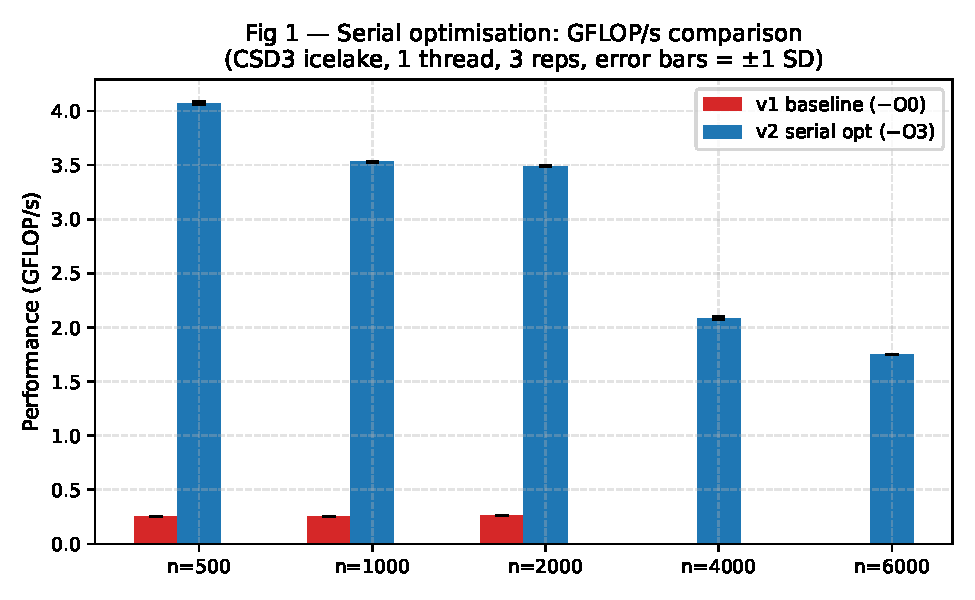
\includegraphics[width=\linewidth]{figures/fig1_serial_gflops.pdf}
    \caption{Serial GFLOP/s (v1, v2, v3\_serial).}
    \label{fig:serial}
  \end{subfigure}\hfill
  \begin{subfigure}[b]{0.48\textwidth}
    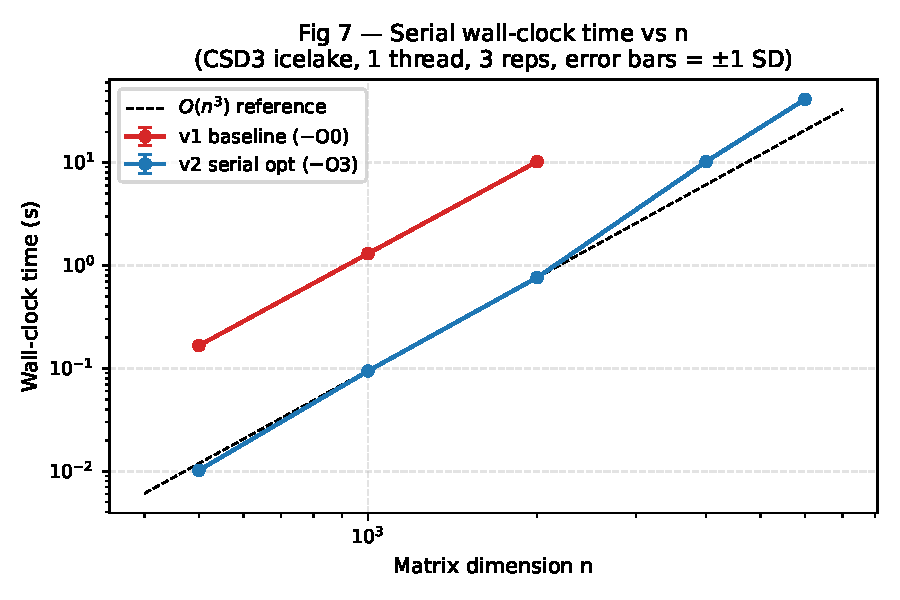
\includegraphics[width=\linewidth]{figures/fig7_serial_time.pdf}
    \caption{Wall-clock time vs.\ $n$ (log-log).}
    \label{fig:serialtime}
  \end{subfigure}
  \caption{Serial performance. CSD3 icelake, 1~thread, \texttt{-O3 -march=native -ffast-math},
           3~reps, error bars $=\pm1$~SD.}
\end{figure}

\subsection{Incremental optimisation}

Figure~\ref{fig:incremental} summarizes the single-thread GFLOP/s at each
development stage for $n=4000$.
The v1$\to$v2 gain (0.26$\to$2.09~GFLOP/s, 8$\times$) comes entirely from
loop reordering and compiler flags.
The v5$\to$v6 gain (2.61$\to$7.21~GFLOP/s, 2.76$\times$) reflects
microarchitectural improvements to the blocked algorithm that are active even
at 1~thread.

\begin{figure}[h]
  \centering
  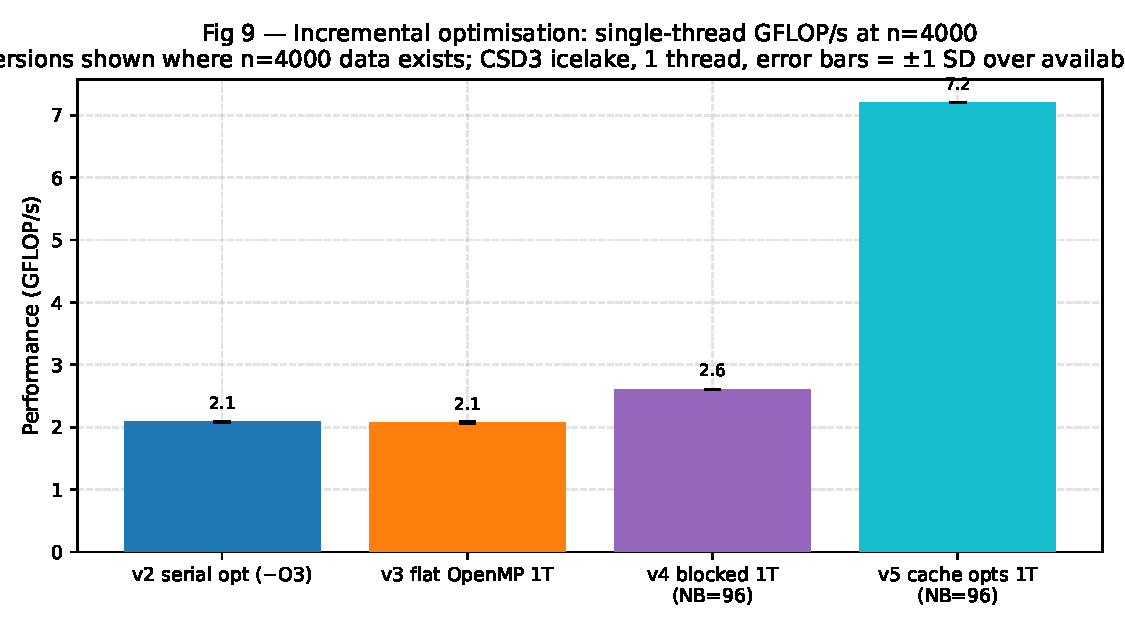
\includegraphics[width=0.72\textwidth]{figures/fig9_incremental.pdf}
  \caption{Incremental optimisation: single-thread GFLOP/s at $n=4000$.
           CSD3 icelake, 1~thread, 3~reps, error bars $=\pm1$~SD.}
  \label{fig:incremental}
\end{figure}

\subsection{Panel-width selection}

Figure~\ref{fig:blocksweep} shows the NB sweep for v5 at $n=8000$, 76~threads.
NB=96 (panel row $= 768$~B, fits in 48~KB L1) peaks at 149.5~GFLOP/s.
Smaller NB increases barrier frequency (NB=64: 125 vs.\ 83 panels).
Larger NB degrades monotonically (NB=128: 137.8; NB=256: 121.7~GFLOP/s)
as L1/L2 pressure from stride-$n$ column accesses grows.

\begin{figure}[h]
  \centering
  \includegraphics[width=0.58\textwidth]{figures/fig8_block_sweep.pdf}
  \caption{GFLOP/s vs.\ panel width NB (v5\_openmp\_blocked, $n=8000$, 76~threads,
           CSD3 icelake, 3~reps).}
  \label{fig:blocksweep}
\end{figure}

\subsection{Strong scaling}

Figures~\ref{fig:scaling}--\ref{fig:efficiency} show GFLOP/s, speedup, and
efficiency for v3\_openmp, v5, and v6 across $n\in\{2000,4000,6000,8000\}$.
Note that v3 data for $n\geq6000$ is incomplete: the single-thread runtime
at $n=6000$ ($\approx$43~s) and $n=8000$ ($\approx$107~s) would have exceeded
the 1-hour INTR limit when multiplied over all 9 thread counts and 3~reps.

\begin{figure}[h]
  \centering
  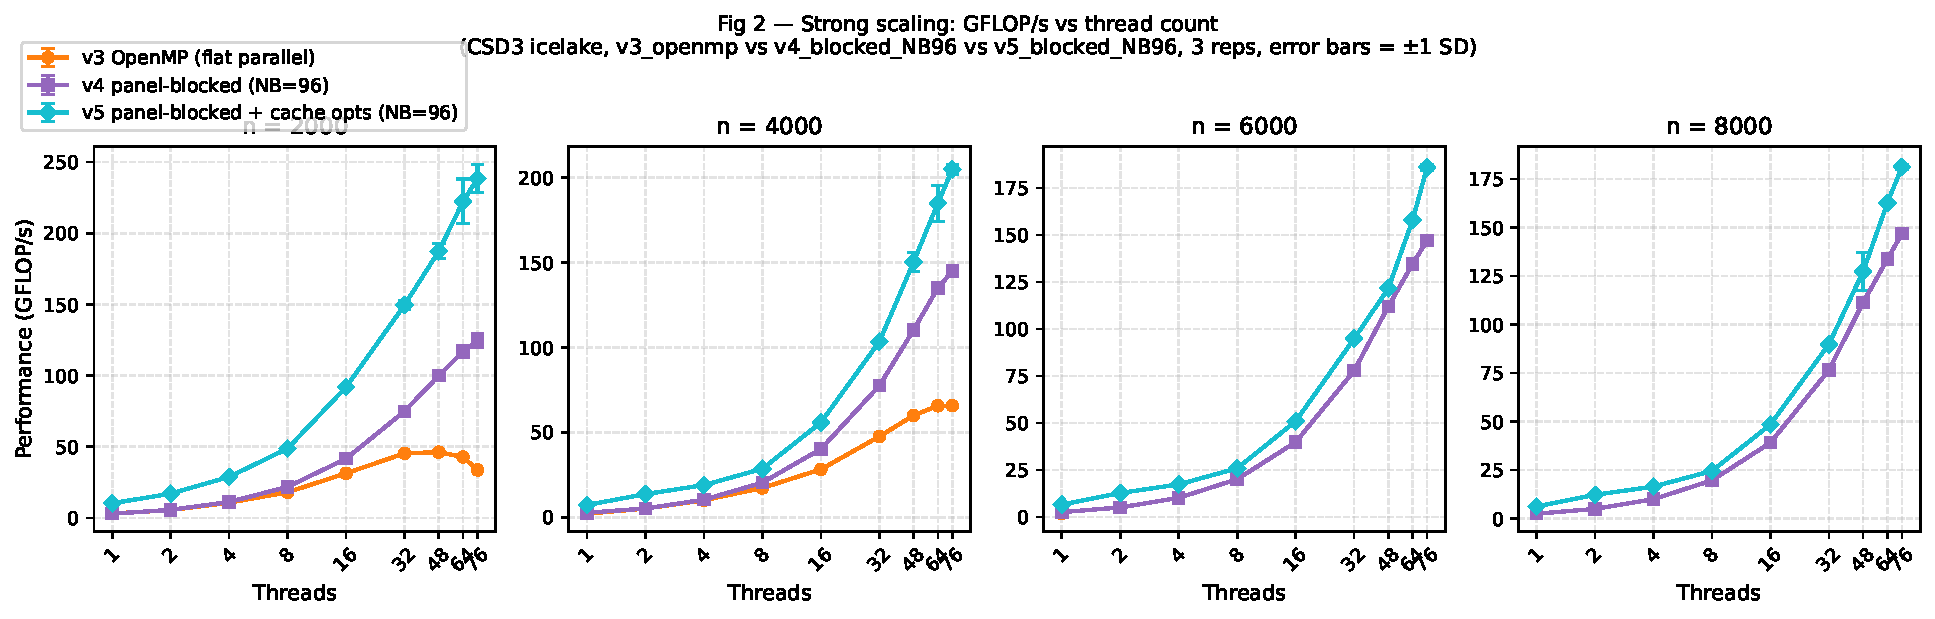
\includegraphics[width=\textwidth]{figures/fig2_scaling_gflops.pdf}
  \caption{Strong scaling: GFLOP/s vs.\ thread count.
           CSD3 icelake, 3~reps, error bars $=\pm1$~SD.}
  \label{fig:scaling}
\end{figure}

\begin{figure}[h]
  \centering
  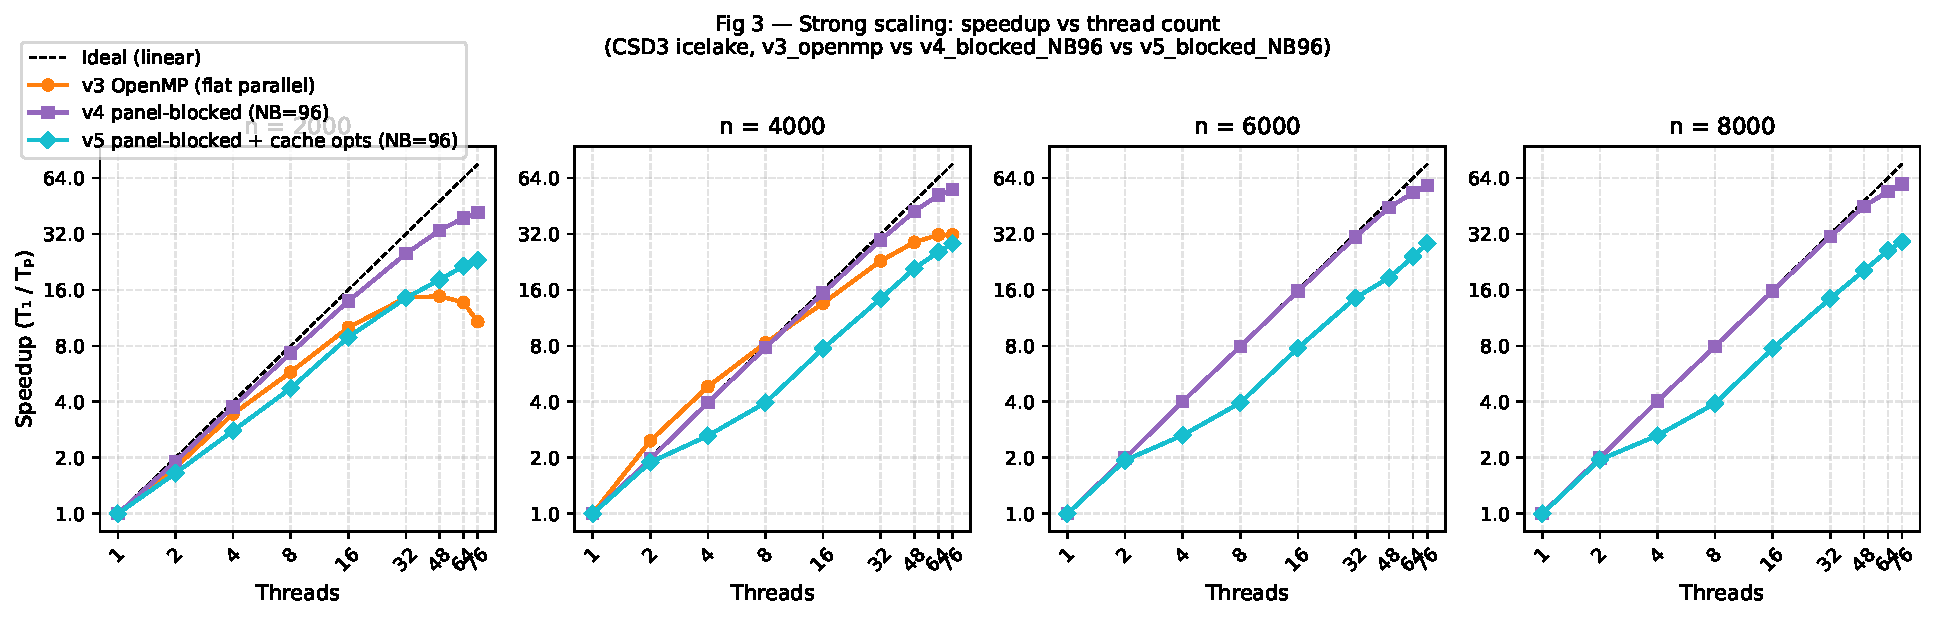
\includegraphics[width=\textwidth]{figures/fig3_scaling_speedup.pdf}
  \caption{Strong scaling: speedup $T_1/T_p$ vs.\ threads (log-log axes).
           Dashed line: ideal linear speedup.
           CSD3 icelake, 3~reps.}
  \label{fig:speedup}
\end{figure}

\begin{figure}[h]
  \centering
  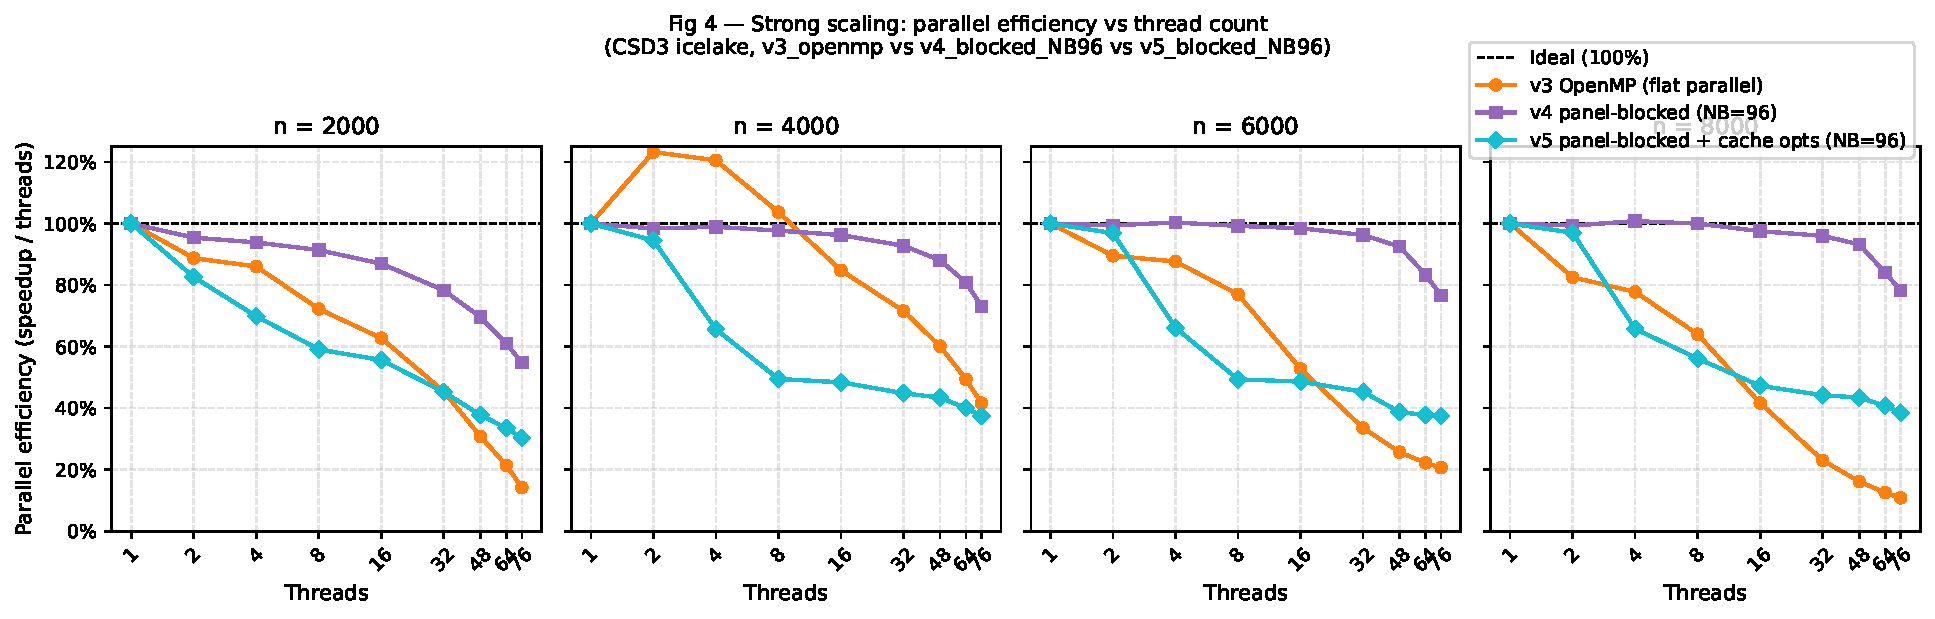
\includegraphics[width=\textwidth]{figures/fig4_scaling_efficiency.pdf}
  \caption{Strong scaling: parallel efficiency $T_1/(p \cdot T_p)$ vs.\ threads.
           CSD3 icelake, 3~reps.}
  \label{fig:efficiency}
\end{figure}

\paragraph{v3 saturation and degradation.}
At $n=2000$, v3 peaks at 46.5~GFLOP/s (48~threads) and degrades to
33.7~GFLOP/s at 76~threads.
Efficiency is only 14.2\% at 76~threads.
The $n=2000$ factorization requires 2000 serial barrier steps; the parallel work
per step ($\approx(n-p)^2/T$) shrinks below constant barrier overhead
as $T$ increases.

\paragraph{v5 near-linear scaling.}
At $n=8000$, v5 achieves 59.4$\times$ speedup and 78.2\% efficiency at
76~threads (146.9~GFLOP/s), with near-linear scaling to 32~threads.
The 83 barrier groups (vs.\ 8000 for v3) provide $96\times$ more computation
per synchronisation event.

\paragraph{v6 microarchitectural gain.}
At $n=8000$, v6 achieves 181.2~GFLOP/s at 76~threads (+23\% over v5).
Its single-thread performance is 2.53$\times$ higher than v5 (6.25 vs.\
2.47~GFLOP/s), driven by OPT-2 (Phase~2 TRSM: L3$\to$L2) and OPT-3
(Phase~3 SYRK: filling both AVX-512 FMA units).
The lower parallel efficiency of v6 (38\%) compared to v5 (78\%) reflects
its stronger single-thread baseline, not worse parallelism: the absolute time
is better at every thread count.

\subsection{Head-to-head comparison at $n=8000$}

\begin{figure}[h]
  \centering
  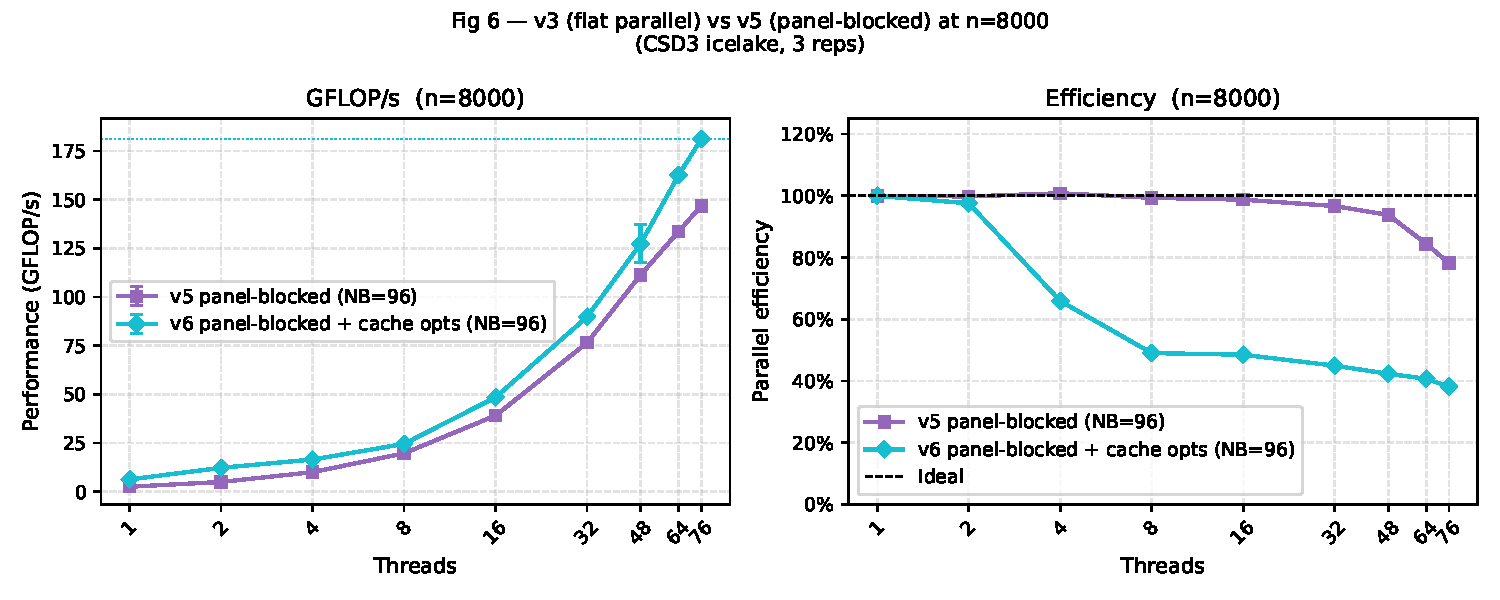
\includegraphics[width=\textwidth]{figures/fig6_v3_vs_v5_n8000.pdf}
  \caption{v3 vs.\ v5 vs.\ v6 at $n=8000$: GFLOP/s (left) and parallel
           efficiency (right). CSD3 icelake, 3~reps.}
  \label{fig:headtohead}
\end{figure}

Figure~\ref{fig:headtohead} provides the direct comparison at $n=8000$.
v3 data is absent (too slow at 1~thread to complete the full scaling study).
At 76~threads, v6 is 3.12$\times$ faster than v3 at $n=4000$ (205.0 vs.\
65.7~GFLOP/s), and v5 is 2.21$\times$ faster.

\subsection{Problem-size scaling}

\begin{figure}[h]
  \centering
  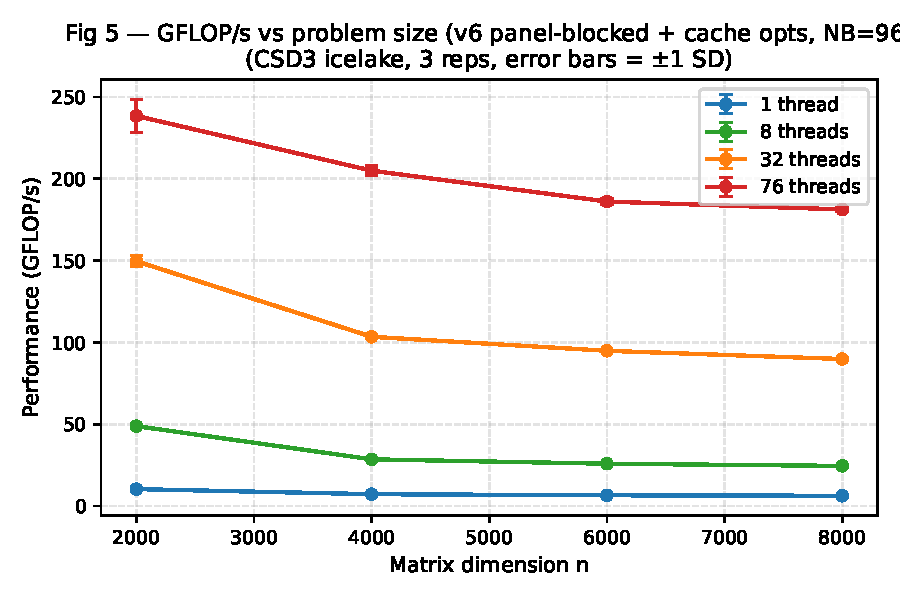
\includegraphics[width=0.62\textwidth]{figures/fig5_problem_size.pdf}
  \caption{GFLOP/s vs.\ $n$ for v6 at selected thread counts.
           CSD3 icelake, 3~reps, error bars $=\pm1$~SD.}
  \label{fig:problemsize}
\end{figure}

Figure~\ref{fig:problemsize} shows v6 GFLOP/s increasing with $n$ at all thread
counts.
At 76~threads, performance grows from 238.8~GFLOP/s at $n=2000$ to
181.2~GFLOP/s at $n=8000$.
The drop at larger $n$ reflects the matrix ($n=8000$: 512~MB) exceeding the
L3 cache (38~MB), shifting the dominant bottleneck toward DRAM bandwidth.

% ======================================================================
\section{Discussion}
% ======================================================================

\paragraph{Amdahl analysis.}
v3's speedup at $n=4000$, 76~threads ($31.6\times$, 41.6\% efficiency) is
limited by the serial fraction of each step (diagonal and column normalization,
$O(n)$ total work vs.\ $O(n^3)$ for the update), amplified by $n=4000$ barrier
calls.
v5 eliminates this bottleneck by making the serial fraction $O(\mathrm{NB}^3)$
per panel and reducing barrier calls to 83.

\paragraph{Super-linear speedup.}
v3 at $n=4000$ shows super-linear speedup at 2--8~threads (8.30$\times$ at
8~threads).
The full matrix (128~MB) exceeds per-socket L3 (38~MB), but with 8~threads the
per-thread active rows fit within L3, reducing DRAM traffic.
This is a cache-capacity effect, not algorithmic super-linearity.

\paragraph{v6 efficiency interpretation.}
The na\"{i}ve reading of v6's 38\% parallel efficiency vs.\ v5's 78\% suggests
v6 parallelizes worse.
This is incorrect: v6's single-thread code is 2.53$\times$ faster, so the
same absolute factorization completes in 0.94~s (v6, 76T) vs.\ 1.16~s (v5, 76T).
Efficiency is a ratio normalized to 1-thread performance; a faster baseline
mechanically lowers the ratio even when absolute throughput improves.

\paragraph{Memory-bound vs.\ compute-bound.}
For small $n$ (2000), the matrix ($n^2 \times 8 = 32$~MB) fits in L3 and the
computation is partially compute-bound; v6 achieves 238.8~GFLOP/s at 76T.
For large $n$ (8000, 512~MB), the working set far exceeds L3 and the problem
becomes bandwidth-limited; v6 achieves 181.2~GFLOP/s.
The NB=96 panel (96 rows $\times$ 8~KB~$=$ 768~KB active SYRK footprint) is
designed to keep the Phase~3 inner loop data in L2, but the full matrix cannot
fit and bandwidth is eventually the ceiling.

% ======================================================================
\section{Conclusion}
% ======================================================================

Starting from a 0.26~GFLOP/s naive baseline, five development stages reach
181~GFLOP/s at 76~threads for $n=8000$ on a single CSD3 icelake node---a
700$\times$ absolute improvement.
Loop reorder and compiler flags contribute 13--16$\times$ on a single core.
Panel blocking removes the synchronisation bottleneck responsible for v3's
degradation at high thread count, achieving 59.4$\times$ speedup and
78.2\% parallel efficiency.
Microarchitectural optimisations (L3$\to$L2 TRSM, dual-FMA-pipeline SYRK,
better load balancing) add a further 2.5$\times$ on each core and
+23\% at full thread count.
Performance is ultimately limited by DRAM bandwidth for large matrices.

\end{document}
